%% nicht vergessen draft raus zu nehmen, um echte Bilder einzubinden und die Problem-Vierecke verschwinden zu lassen
\documentclass[11pt,a4paper,oneside,svgnames]{report}

\usepackage[utf8]{inputenc}
\usepackage[T1]{fontenc}
\usepackage{lmodern}
\usepackage{eurosym}
\usepackage[british]{babel}

\usepackage{ae}
\usepackage{hyperref}
\usepackage{float}
\usepackage[table]{xcolor}
\usepackage{colortbl}
\usepackage{multirow}
\usepackage{tabularx}
\usepackage{graphicx}
\usepackage{tikz}
\usepackage{kpfonts}
\usepackage[explicit]{titlesec}
\usepackage[acronym,nonumberlist,style=tree]{glossaries}
\usepackage{amssymb}
\usepackage[left=3.65cm,right=3.65cm,top=3cm,bottom=3cm]{geometry}

\usepackage{fancyhdr}
\pagestyle{fancy}

\fancypagestyle{plain}{
    \fancyhf{}
	\fancyfoot[LO,LE]{M. A. Harnos, J. Rapp, C. Schulz}
	\cfoot{}
	\rfoot{\thepage}
    \renewcommand{\headrulewidth}{0pt}
	\renewcommand{\footrulewidth}{0.4pt}
}

%BEGIN Header and Footer Design
\rhead{}
\fancyhead[LO,LE]{\slshape \leftmark}
\fancyfoot[LO,LE]{M. A. Harnos, J. Rapp, C. Schulz}
\cfoot{}
\rfoot{\thepage}
\renewcommand{\headrulewidth}{0.4pt}
\renewcommand{\footrulewidth}{0.4pt}
%END Header and Footer Design

%BEGIN Chapter Definition

\makeatletter
\def\thickhrulefill{\leavevmode \leaders \hrule height 1ex \hfill \kern \z@}
\def\@makechapterhead#1{%
  \vspace*{0\p@}%
  {\parindent \z@ \raggedleft \reset@font
            \scshape \@chapapp{} \thechapter
        \par\nobreak
        \interlinepenalty\@M
    \Huge \bfseries #1\par\nobreak
    %\vspace*{1\p@}%
    \hrulefill
    \par\nobreak
    \vskip 20\p@
  }}
\def\@makeschapterhead#1{%
  \vspace*{0\p@}%
  {\parindent \z@ \raggedleft \reset@font
            \scshape \vphantom{\@chapapp{} \thechapter}
        \par\nobreak
        \interlinepenalty\@M
    \Huge \bfseries #1\par\nobreak
    %\vspace*{1\p@}%
    \hrulefill
    \par\nobreak
    \vskip 20\p@
  }}

%END Chapter Definition

%BEGIN Title Definition

\makeatletter
\def\thickhrulefill{\leavevmode \leaders \hrule height 1pt\hfill \kern \z@}
\renewcommand{\maketitle}{\begin{titlepage}%
    \let\footnotesize\small
    \let\footnoterule\relax
    \parindent \z@
    \reset@font
    \null\vfil
    \begin{flushleft}
      \huge \@title
    \end{flushleft}
    \par
    \hrule height 4pt
    \par
    \begin{flushright}
      \LARGE \@author \par
    \end{flushright}
    \vskip 60\p@
    \vfil\null
  \end{titlepage}%
  \setcounter{footnote}{0}%
}

%END Title Definition

%Verschissener rotierter Text für verschissene Tabelle 14.1/2
\makeatletter
\newsavebox\zzz
\def\mystrut{%
\dimen@\wd\zzz
\divide\dimen@\thr@@
\advance\dimen@-\dp\@arstrutbox
\rule\z@\dimen@}

\def\rotatezzz{%
\rotatebox{90}{\rlap{\kern-\dp\@arstrutbox\usebox\zzz}}}
%END Verschissener rotierter Text

\makeatother
\title{Specification Sheet for Project ``BookExpress''}
\author{Marc A. Harnos\\ {mharnos@gmail.com} \and Joscha Rapp\\ {jraxxo@gmail.com} \and Christian Schulz\\ {crs.s@gmx.net}}
\author{Marc A. Harnos\\ Joscha Rapp\\ Christian Schulz}
\date{October 2012}

\definecolor{tableHead}{HTML}{5393B7}
\definecolor{tableEven}{HTML}{DAF1FF}
\definecolor{tableOdd}{HTML}{ADD0E5}
\definecolor{tableFoot}{HTML}{5393B7}

\definecolor{linkcolour}{rgb}{0,0.2,0.6}

\hypersetup{colorlinks,breaklinks,urlcolor=linkcolour,linkcolor=linkcolour}
\renewcommand{\arraystretch}{1.25}

\makeglossaries

\newglossaryentry{pin}{name=PIN,description={Personal Identification Number},plural=PINs, first={Personal Identification Number (PIN)}}

\newacronym{led}{LED}{light-emitting diode}
\newacronym{html}{HTML}{Hypertext Markup Language}
\newacronym{css}{CSS}{Cascade Stylesheet}
\newacronym{js}{JS}{JavaScript}
\newacronym{ie}{IE}{InternetExplorer}
\newacronym{vm}{VM}{Virtual Machine}
\newacronym{ide}{IDE}{Integrated Development Environment}


\begin{document}

\maketitle
\clearpage
\tableofcontents
\clearpage

\chapter*{Document History}

\begin{table}[H]
\centering
\begin{tabular}{|p{3.8cm}|p{2cm}|p{5.5cm}|p{1.2cm}|}
\hline 
Editor(s) & Date & Purpose of Editing & Version \\ 
\hline 
Harnos, Rapp, Schulz & 2012-09-13 & Added Purpose/Aims of the Product & v0.2 \\ 
\hline
Harnos, Schulz & 2012-09-13 & Added Usage of the Product, Product Overview, Product Functions & v0.4 \\ 
\hline
Rapp, Schulz & 2012-09-14 & Added Product Data, Product Performance & v0.8 \\ 
\hline 
Harnos, Rapp & 2012-09-15 & Added Quality Requirements, Amendments & v1.0 \\ 
\hline 
\end{tabular}
\caption{Document History Table}
\label{tab:document-history}
\end{table}

\chapter{Purpose/Aims of the Product}
The goal of the project is to create a software that will drastically reduce the amount of work the employees of "BookExpress" spend on logistics and administration, thus speeding up the processes and making sure that every customer gets his or her orders as soon as possible, within the specified timeframe (24 hours). The current IT system is not as flexible or comfortable as it should be - as a result the business processes, such as maintaining a stock database that is consistent as well as up-to-date, are overly complex and time-consuming. The user interface has to be intuitive and performant, relieving the employees of a lot of administrative work and quite possibly reducing the time that new employees need to become familiar with it. By establishing a direct connection to the customers and publishers, all processes can be handled faster - furthermore, as almost all processes are handled by the software, automatic tracking of orders and deliveries is possible, giving estimates of delivery dates/hours. This new IT system will also need a renewal of the existent hardware as it is severely outdated. 
\\
\chapter{Usage of the Product}
The new IT system will be used by employees of BookExpress as well as the customers and publishers themselves. With the new system, customers will be able to submit orders automatically, depending on their demands, e.g. if their stock is below a certain threshold or they need to get a book for a final customer. The publisher on the other hand can push updates in their stock in realtime - as soon as a new book is available, it can be ordered from BookExpress. Furthermore, the new user experience will be much more modern and streamlined - instead of the old text-based system, all users will be able to use a modern, web-based interface which can even be accessed on mobile devices such as smartphones and tablets, thus increasing the flexibility of employees and customers even more.
\\
\clearpage
\chapter{Product Overview}

\begin{figure}[H]
 \begin{center}
  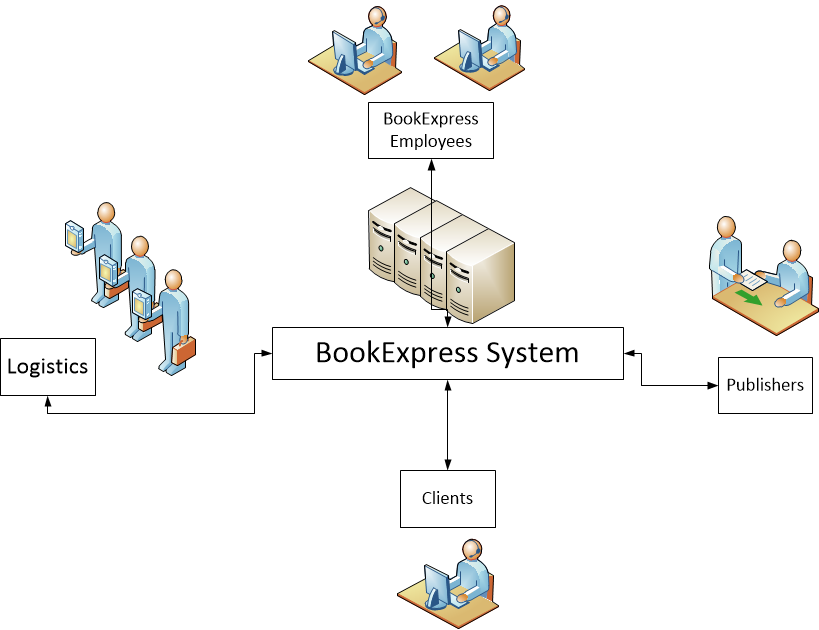
\includegraphics[width=\textwidth]{ProductOverview.png}
 \end{center}
 \caption{The Product Overview}
\end{figure}

\chapter{Product Functions}

\rowcolors{1}{tableEven}{tableOdd}
\begin{table}[H]
\centering
\begin{tabular}{p{1.5cm}p{3cm}p{8cm}}
\cellcolor{white}/SF10/	& \textbf{Process}	& Register Publisher or Book Shop (client)\\
\cellcolor{white}		& \textbf{Actor(s)} & Publishers \\
\cellcolor{white}		& \textbf{Description}	 & Publishers can update their inventory list (i.e. the list of available books) either via mail or using the direct connection over the web-based interface. \\
\end{tabular}
\caption{/SF10/ Inventory maintenance (Publisher)}
\end{table}

\begin{table}[H]
\centering
\begin{tabular}{p{1.5cm}p{3cm}p{8cm}}
\cellcolor{white}/SF20/	& \textbf{Process}	& BookExpress Order \\
\cellcolor{white}		& \textbf{Actor(s)} & Employee \\
\cellcolor{white}		& \textbf{Description}	 &  The Employee orders a number of Books from the publisher.\\
\end{tabular}
\caption{/SF20/ BookExpress Order}
\end{table}

\begin{table}[H]
\centering
\begin{tabular}{p{1.5cm}p{3cm}p{8cm}}
\cellcolor{white}/SF30/	& \textbf{Process}	& Book Store Order \\
\cellcolor{white}		& \textbf{Actor(s)} &  Book Store Employee \\
\cellcolor{white}		& \textbf{Description}	 &  The Book Store orders a book from BookExpress. This can either happen through a constant connection where every order is individually processed or the store can choose to collect orders internally and send them as one big order every day. \\
\end{tabular}
\caption{/SF30/ Book Store Order}
\end{table}

\begin{table}[H]
\centering
\begin{tabular}{p{1.5cm}p{3cm}p{8cm}}
\cellcolor{white}/SF40/	& \textbf{Process}	&  Stock Update (BookExpress)\\
\cellcolor{white}		& \textbf{Actor(s)} &  Stock Employee  \\
\cellcolor{white}		& \textbf{Description}	 & The employee in charge of the stock checks the availability of all books and updates the stock accordingly. \\
\end{tabular}
\caption{/SF40/  Stock Update (BookExpress)}
\end{table}


\begin{table}[H]
\centering
\begin{tabular}{p{1.5cm}p{3cm}p{8cm}}
\cellcolor{white}/SF50/	& \textbf{Process}	& Cancel Order \\
\cellcolor{white}		& \textbf{Actor(s)} &   Book Store Employee\\
\cellcolor{white}		& \textbf{Description}	 &  The employee at the book store can cancel the order if it hasn't been shipped yet. \\
\end{tabular}
\caption{/SF50/ Cancel Order}
\end{table}

\begin{table}[H]
\centering
\begin{tabular}{p{1.5cm}p{3cm}p{8cm}}
\cellcolor{white}/SF60/	& \textbf{Process}	&  Tracking System \\
\cellcolor{white}		& \textbf{Actor(s)} &  Book Store Employee\\
\cellcolor{white}		& \textbf{Description}	 &  The employee at the book store can look up at which stage his order is right now, e.g. processing or shipping to BookExpress/the book store.\\
\end{tabular}
\caption{/SF60/ Tracking System }
\end{table}

\chapter{Product Data}

\begin{table}[H]
\centering
\begin{tabular}{p{1.5cm}p{3cm}p{8cm}}
\cellcolor{white}/SD10/	& \textbf{Data}	& Book Data - ISBN, UPC/EAN, Title/Author, Publisher, Availability... \\
\cellcolor{white}	 & \textbf{Maximum)} &  1,500,000\\
\end{tabular}
\caption{/SD10/ Product Data }
\end{table}

\begin{table}[H]
\centering
\begin{tabular}{p{1.5cm}p{3cm}p{8cm}}
\cellcolor{white}/SF40/	& \textbf{Data}	&  Book Store Data - PIN/Password, Name/Address, Order Type (Continuous / Summary), Contact Data \\
\cellcolor{white}		& \textbf{Maximum)} &  10,000\\
\end{tabular}
\caption{/SF40/ Product Data}
\end{table}

\begin{table}[H]
\centering
\begin{tabular}{p{1.5cm}p{3cm}p{8cm}}
\cellcolor{white}/SD30/	& \textbf{Data}	& Publisher Data - Account Name/Password, Name/Address, Stock-keeping Type (Direct/Written Notes), Contact Data \\
\cellcolor{white}		& \textbf{Maximum)} & 15,000 \\
\end{tabular}
\caption{/SD30/ Product Data}
\end{table}

\begin{table}[H]
\centering
\begin{tabular}{p{1.5cm}p{3cm}p{8cm}}
\cellcolor{white}/SD40/	& \textbf{Data}	& Order Data - ISBN, Amount, Price, Current State\\
\cellcolor{white}		& \textbf{Maximum)} & 500,000 \\
\end{tabular}
\caption{/SD40/ Product Data}
\end{table}

\begin{table}[H]
\centering
\begin{tabular}{p{1.5cm}p{3cm}p{8cm}}
\cellcolor{white}/SD50/	& \textbf{Data}	& Truck Fleet Data - Driver, Registration Number \\
\cellcolor{white}		& \textbf{Maximum)} &  1,000 \\
\end{tabular}
\caption{/SD50/ Product Data}
\end{table}

\chapter{Product Performance}

\begin{table}[H]
\centering
\begin{tabular}{p{1.5cm}p{11cm}}
\cellcolor{white}/SP10/ & The Web Interface has to be comfortably reachable from computers and tablets/smartphones, it has to be intuitive and interactive.\\
\end{tabular}
\caption{/SP10/ Product Performance}
\end{table}

\begin{table}[H]
\centering
\begin{tabular}{p{1.5cm}p{11cm}}
\cellcolor{white}/SP20/ & The amount of transferred data should be minimal. \\
\end{tabular}
\caption{/SP20/ Product Performance}
\end{table}

\begin{table}[H]
\centering
\begin{tabular}{p{1.5cm}p{11cm}}
\cellcolor{white}/SP30/ & If either a book store or an employee submits an order, there has to be an immediate notification if said order was successful.\\
\end{tabular}
\caption{/SP30/ Product Performance}
\end{table}

\begin{table}[H]
\centering
\begin{tabular}{p{1.5cm}p{11cm}}
\cellcolor{white}/SP40/ & We need a highly reliable infrastructure, for an uptime of 99\% or preferably more. \\
\end{tabular}
\caption{/SP40/ Product Performance}
\end{table}

\begin{table}[H]
\centering
\begin{tabular}{p{1.5cm}p{11cm}}
\cellcolor{white}/SP50/ & The system has to be able to process up to 2000 orders submitted at once. \\
\end{tabular}
\caption{/SP50/ Product Performance}
\end{table}

\begin{table}[H]
\centering
\begin{tabular}{p{1.5cm}p{11cm}}
\cellcolor{white}/SP60/ & If a book is running low on stock, the system shall automatically try to order a certain amount of that book from the publisher.  If that fails for whatever reason, the employees shall be notified. \\
\end{tabular}
\caption{/SP60/ Product Performance}
\end{table}

\chapter{Quality Requirements}
As stated before, the system has to be extremely reliable as it is very important for every customer. The interface has to be highly performant and intuitive to provide a comfortable ordering experience for the customers as well as the employees. The complete software has to be engineered according to the guidelines defined in ISO/IEC 25000. As BookExpress cannot afford a downtime of any kind, the transition from the old system to the new one has to be very smooth. If a restart is required, it is to be executed during the night of a holiday, if possible. Additionally, we need a dedicated support team for hardware and software to ensure a flawless performance if anything goes wrong.
\chapter{Amendments}
To enhance the customer experience and speed up processes even more, every (bigger) customer will be asked to upgrade to a direct line instead of summary order. Moreover, The tracking system shall be implemented by getting direct GPS data from the truck that is transporting the shipment, thus providing truly accurate estimates of the time of delivery. The web interface has to be thoroughly tested in the currently important browsers(Chrome, FireFox, Opera, Safari, IE8+, mobile Browsers (Opera mobile, iOS (Safari), Chrome, Android(Dolphin))).
\chapter{Glossary}
\begin{tabbing}
\hspace{3cm}\=\kill
	Customer  \> Book Store with an account\\
	\\
	PIN       \> Personal Identification Number, used to identify the customer\\
	\\
	 
\end{tabbing} 

\listoffigures\addcontentsline{toc}{section}{List of Figures}
\listoftables\addcontentsline{toc}{section}{List of Tables}

\end{document}
